%%%%%%%%%%%%%%%%%%%%%%%%%%%%%%%%%%%%%%%%%
% Short Sectioned Assignment LaTeX Template Version 1.0 (5/5/12)
% This template has been downloaded from: http://www.LaTeXTemplates.com
% Original author:  Frits Wenneker (http://www.howtotex.com)
% License: CC BY-NC-SA 3.0 (http://creativecommons.org/licenses/by-nc-sa/3.0/)
%%%%%%%%%%%%%%%%%%%%%%%%%%%%%%%%%%%%%%%%%

%----------------------------------------------------------------------------------------
%	PACKAGES AND OTHER DOCUMENT CONFIGURATIONS
%----------------------------------------------------------------------------------------

\documentclass[12pt]{article} % A4 paper

% ---- Entrada y salida de texto -----

\usepackage[T1]{fontenc} % Use 8-bit encoding that has 256 glyphs
\usepackage[utf8]{inputenc}
%\usepackage{fourier} % Use the Adobe Utopia font for the document - comment this line to return to the LaTeX default

% ---- Idioma --------

\usepackage[spanish, es-tabla]{babel} % Selecciona el español para palabras introducidas automáticamente, p.ej. "septiembre" en la fecha y especifica que se use la palabra Tabla en vez de Cuadro

% ---- Otros paquetes ----

\usepackage{url} % ,href} %para incluir URLs e hipervínculos dentro del texto (aunque hay que instalar href)
\usepackage{amsmath,amsfonts,amsthm} % Math packages
%\usepackage{graphics,graphicx, floatrow} %para incluir imágenes y notas en las imágenes
\usepackage{graphics,graphicx, float} %para incluir imágenes y colocarlas
\usepackage{algpseudocode}
\usepackage{algorithmicx}
\usepackage{algorithm}
\usepackage{dirtree}
\usepackage{booktabs}
\usepackage{multirow}
\usepackage[table,xcdraw]{xcolor}
\usepackage{caption}
\captionsetup[table]{position=bottom} 

% Para hacer tablas comlejas
%\usepackage{multirow}
%\usepackage{threeparttable}

%\usepackage{sectsty} % Allows customizing section commands
%\allsectionsfont{\centering \normalfont\scshape} % Make all sections centered, the default font and small caps

\usepackage{fancyhdr} % Custom headers and footers
\pagestyle{fancyplain} % Makes all pages in the document conform to the custom headers and footers
\fancyhead{} % No page header - if you want one, create it in the same way as the footers below
\fancyfoot[L]{} % Empty left footer
\fancyfoot[C]{} % Empty center footer
\fancyfoot[L]{\thepage} % Page numbering for right footer
\renewcommand{\headrulewidth}{0pt} % Remove header underlines
\renewcommand{\footrulewidth}{0pt} % Remove footer underlines
%\setlength{\headheight}{-10pt} % Customize the height of the header

\numberwithin{equation}{section} % Number equations within sections (i.e. 1.1, 1.2, 2.1, 2.2 instead of 1, 2, 3, 4)
\numberwithin{figure}{section} % Number figures within sections (i.e. 1.1, 1.2, 2.1, 2.2 instead of 1, 2, 3, 4)
\numberwithin{table}{section} % Number tables within sections (i.e. 1.1, 1.2, 2.1, 2.2 instead of 1, 2, 3, 4)

\setlength\parindent{0.7cm} % Removes all indentation from paragraphs - comment this line for an assignment with lots of text
\setlength\parskip{0.3cm}

\newcommand{\horrule}[1]{\rule{\linewidth}{#1}} % Create horizontal rule command with 1 argument of height

\let\stdpart\part
\renewcommand\part{\newpage\stdpart}
\newcommand{\pluseq}{\mathrel{+}=}

\usepackage[
    a4paper,
    left=2.8cm,
    right=2.5cm,
    top=3cm,
    bottom=3cm
]{geometry}


%----------------------------------------------------------------------------------------
%	TÍTULO Y DATOS DEL ALUMNO
%----------------------------------------------------------------------------------------

\title{	
\normalfont \normalsize 
\huge{\textbf{Metaheurísticas (Curso 2021-2022)}\linebreak \linebreak Grado en Ingeniería Informática \\ Universidad de Granada} \\ [23pt] % Your university, school and/or department name(s)

\begin{figure}[H] %con el [H] le obligamos a situar aquí la figura
    \centering
        
\includegraphics[scale=0.4]{img/ugr.png}
\end{figure}

\horrule{0.5pt} \\[0.4cm] % Thin top horizontal rule
\huge Práctica 2: Técnicas de Búsqueda basadas en Poblaciones \linebreak \linebreak% The assignment title
\LARGE Problema a: Mínima Dispersión Diferencial
\horrule{2pt} \\[0.5cm] % Thick bottom horizontal rule
\vspace{0.7cm}

\Large{Pedro Bedmar López - 75935296Z} \\
\Large{pedrobedmar@correo.ugr.es} \linebreak

\large Grupo de prácticas 3 - Martes 17:30-19:30

}

\date{}

%----------------------------------------------------------------------------------------
% DOCUMENTO
%----------------------------------------------------------------------------------------

\begin{document}

\clearpage
\maketitle % Muestra el Título
\thispagestyle{empty}

\newpage %inserta un salto de página

\tableofcontents % para generar el índice de contenidos

\newpage



%----------------------------------------------------------------------------------------
%	Cuestión 1
%----------------------------------------------------------------------------------------

\part{Formulación del problema}

Sea $G = (V,E)$ un grafo completo no dirigido donde $V$, de tamaño $n$, es el conjunto de vértices que lo forman y $E$ es el conjunto de las aristas que unen estos vértices. Este grafo es un grafo ponderado, ya que cada una de las aristas $e_{u,v} \in E$ lleva asociada un peso que representa la distancia $d_{u,v}$ entre dos vértices $u,v \in V$.

La dispersión es una medida que se puede aplicar en este dominio, donde dado un subconjunto $S \subset V$ de tamaño $m$ se mide cómo de homogéneas son las distancias entre los vértices que forman $S$. Una de las aplicaciones más importantes de las Ciencias de la Computación consiste en optimizar valores como éste, maximizando o minimizando el resultado que devuelve una \textbf{función objetivo}. 

En esta práctica queremos minimizar su valor, obteniendo la mínima dispersión. Este problema tiene un gran paralelismo con problemas reales, como puede ser la organización del género en almacenes, donde minimizar la dispersión de la mercancía reduce los costes. Por tanto, si resolvemos este problema de forma teórica es trivial aplicar la solución en estos casos.

Anteriormente he definido la dispersión de una forma muy genérica, sin entrar en su formalización. Y es que se puede definir de diferentes formas, teniendo en cuenta la dispersión media de los elementos del conjunto $S$ o utilizando los valores extremos (máximos y mínimos) en éste. Esta segunda opción se define formalmente como:
\begin{align*}
    diff(S) = max_{i \in S} \{ \sum_{j \in S} d_{i,j}\} - min_{i \in S} \{ \sum_{j \in S} d_{i,j}\}
\end{align*}

Utilizando esta definición de dispersión como función objetivo obtenemos lo que se conoce como \textbf{Problema de la Mínima Dispersión Diferencial (MDD)}, es decir: 
\begin{align*}
    S^{*} = {arg min}_{S \subset V} diff(S)
\end{align*}


\part{Descripción de la aplicación de los algoritmos}
En esta segunda práctica de la asignatura implementamos y comparamos el rendimiento de algoritmos de búsqueda basados en poblaciones, en concreto algoritmos \textbf{Genéticos} y \textbf{Meméticos}. Antes de describirlos, vamos a comentar información común a ambos.


\section{Datos utilizados}
Los datos que necesitamos para analizar el comportamiento de los algoritmos en este problema no son muy complejos. En cada posible instancia se necesita conocer el valor $n$ indicando el número de puntos que contiene el dataset, el valor $m < n$ indicando cuantos puntos se quieren escoger de forma que se minimice la dispersión en esos $m$ puntos y la matriz $d$ con tamaño $n \times n$, simétrica y con valor 0 en su diagonal, que contiene las distancias entre cada uno de los $n$ puntos del dataset. En definitiva, se necesita conocer el grafo $G$.

En total, en los experimentos utilizamos 50 instancias diferentes con datos extraídos del dataset \textbf{GKD}. Las instancias toman valores $n \in \{25,50,100,125,150\}$ y $m \in [2,45]$.

\section{Representación de soluciones}

El conjunto $V$ descrito en la formulación del problema coincide con $n$ en tamaño. Al contrario que en la práctica anterior, una posible solución $S$ puede representarse de dos formas diferentes según el punto de ejecución en que se encuentre el algoritmo.

En la búsqueda local del algoritmo memético, la solución se representa de la misma forma que en la práctica anterior para poder reutilizar el código, siendo $S$ es una solución válida si:
\begin{itemize}
    \item $|S| = m$
    \item $S \subset V$
\end{itemize}
Y por tanto, $m < n$. Estamos ante una representación entera donde los índices de los vértices que forman la solución son recogidos por $S$. Por ejemplo $S = \{3,7,2\}$ representa que los vértices con índice 3, 7 y 2 forman una solución al problema.

En cambio, para la mayor parte del algoritmo memético y todo el genético, la representación que se utiliza es binaria. Para diferenciar la representación anterior de ésta, vamos a nombrarla $S_b$ en vez de $S$. Cumple las siguientes condiciones:
\begin{itemize}
    \item $|S_b| = n$
    \item count(1, $S_b$) = $m$, donde count(1, $S_b$) devuelve el número de 1s en $S_b$.
    \item $S_b = [x | x \in \{0,1\}]$
\end{itemize}
El orden de los valores en $S_b$ importa, cada uno representa un vértice del grafo, por lo que se implementará como un vector y no como un conjunto. Por ejemplo, $S_b = [1,0,0,1,0,1]$ representa que los vértices 1, 4 y 6 del grafo forman parte de la solución pero el resto no.




\section{Función objetivo}

Como hemos comentado al describir el problema, la función objetivo a minimizar se define como:
\begin{align*}
    diff(S) = max_{i \in S} \{ \sum_{j \in S} d_{i,j}\} - min_{i \in S} \{ \sum_{j \in S} d_{i,j}\}
\end{align*}

\noindent En el caso de utilizar representación entera para las posibles soluciones, el pseudocódigo quedaría de la siguiente forma:
\begin{algorithm}[H]
    \caption{Función objetivo, implementación para la representación entera}
\begin{algorithmic}
\State $max \gets -\infty$
\State $min \gets \infty$
\For{$s \in S$}
    \State $distance \gets \sum_{s2 \in S} d_{s,s2}$
    \If{$distance > max$}
        \State $max \gets distance$
    \EndIf
    \If{$distance < min$}
        \State $min \gets distance$
    \EndIf
\EndFor
\State \textbf{return} $max - min$
\end{algorithmic}
\end{algorithm}

En el algoritmo de Búsqueda Local, no se utiliza directamente esta implementación de la función objetivo. Esto se debe a que es costosa, en concreto tiene una complejidad computacional de $O(n^2)$. Utilizamos una versión factorizada de la función, que reutiliza cálculos de iteraciones previas para actualizar el valor de la dispersión. De esta forma, obtenemos una complejidad de $O(n)$.

En las situaciones en las que las soluciones se representen de forma binaria, el pseudocódigo de la función objetivo quedaría así:
\begin{algorithm}[H]
    \caption{Función objetivo, implementación para la representación binaria}
\begin{algorithmic}
\State $max \gets -\infty$
\State $min \gets \infty$
\For{$i \in S_b$} \Comment{Donde $i$ indica la posición en el vector $S_b$}
    \If{$S_b[i] == 1$}
        \State $distance \gets 0$
        \State
        \For{$j \in S_b$}
            \If{$S_b[j] == 1$} \Comment{Donde $j$ indica la posición en el vector $S_b$}
                \State $distance += d_{i,j}$
            \EndIf
        \EndFor
        \State
        \If{$distance > max$}
            \State $max \gets distance$
        \EndIf
        \If{$distance < min$}
            \State $min \gets distance$
        \EndIf
    \EndIf
\EndFor
\State \textbf{return} $max - min$
\end{algorithmic}
\end{algorithm}

\section{Operadores comunes}

En esta sección se describen los operadores comunes a los diferentes algoritmos.

\subsection{Generador de soluciones aleatorias}
\begin{algorithm}[H]
    \caption{Generador de soluciones aleatorias en representación binaria.}
\begin{algorithmic}
\Procedure{generateRandomSolution}{}
    \State $individual \leftarrow [ \, ]$
    \For{$i = 0$ \textbf{to} $m-1$}
        \State $individual += \{true\}$ \Comment{Insertamos un $true$ al final del vector}
    \EndFor
    \For{$i = 0$ \textbf{to} $n-m-1$}
        \State $individual += \{false\}$
    \EndFor
    \State shuffle($individual$)
    \State \textbf{return} $individual$
\EndProcedure
\end{algorithmic}
\end{algorithm}


\subsection{Mecanismos de selección}
\begin{algorithm}[H]
    \caption{Mecanismo de selección del algoritmo genético generacional. Toma como argumentos un vector que contiene la población de individuos y otro vector que contiene la dispersión de cada individuo. Devuelve la población que contiene a los padres, de tamaño 50.}
\begin{algorithmic}
\Procedure{generationalSelectionOperator}{popul, populDisp}
    \State $parentsPopul \leftarrow [ \, ]$
    \State $parentsPopulDisp \leftarrow [ \, ]$
    \State
    \For{$i = 0$ \textbf{to} $49$}
        \State $firstRandElem \leftarrow $rand($0,49$)
        \State $secondRandElem \leftarrow $rand($0,49$) \Comment Debe de ser diferente a $firstRandElem$
        \State
        \State $bestRandElem \leftarrow firstRandElem$
        \If{$populDisp[bestRandElem]>populDisp[secondRandElem]$}
            \State $bestRandElem \leftarrow secondRandElem$
        \EndIf
        \State
        \State $parentsPopul += \{popul[bestRandElem]\}$
        \State $parentsPopulDisp += \{populDisp[bestRandElem]\}$
    \EndFor
    \State
    \State \textbf{return} $parentsPopul, parentsPopulDisp$
\EndProcedure
\end{algorithmic}
\end{algorithm}

\begin{algorithm}[H]
    \caption{Mecanismo de selección del algoritmo genético estacionario. Toma como argumentos un vector que contiene la población de individuos y otro vector que contiene la dispersión de cada individuo. Devuelve el índice en la población de los dos individuos elegidos como padres.}
\begin{algorithmic}
\Procedure{stationarySelectionOperator}{popul, populDisp}
    \State $parents \leftarrow [ \, ]$
    \State 
    \State $firstRandElem \leftarrow$ rand($0$, $49$) 
    \State $secondRandElem \leftarrow$ rand($0$, $49$) \Comment Debe de ser diferente a $firstRandElem$
    \State $parent1Index \leftarrow firstRandElem$
    \If{$populDisp[parent1Index] > populDisp[secondRandElem]$}
        \State $parent1Index \leftarrow secondRandElem$
    \EndIf
    \State 
    \State $firstRandElem \leftarrow$ rand($0$, $49$) 
    \State $secondRandElem \leftarrow$ rand($0$, $49$) \Comment Debe de ser diferente a $firstRandElem$
    \State $parent2Index \leftarrow firstRandElem$
    \If{$populDisp[parent2Index] > populDisp[secondRandElem]$}
        \State $parent2Index \leftarrow secondRandElem$
    \EndIf
    \State
    \State \textbf{return} $parent1Index, parent2Index$
\EndProcedure
\end{algorithmic}
\end{algorithm}


\subsection{Operadores de cruce}
\begin{algorithm}[H]
    \caption{Operador de cruce uniforme. Cruza dos individuos, generando un hijo que mantiene los genes comunes y asigna uno valor aleatorio en aquellos no comunes. Si el hijo no es factible, se repara. Devuelve este hijo.}
\begin{algorithmic}
\Procedure{uniformCrossoverOperator}{parent1, parent2}
    \State $child \leftarrow parent1$
    \State
    \For{$i = 0$ \textbf{to} $n-1$}
        \If{$parent1[i] != parent2[i]$}
            \State $child[i] \leftarrow$ rand($0,1$)
        \EndIf
    \EndFor
    \State
    \State $countNbTrues \leftarrow 0$
    \For{$i = 0$ \textbf{to} $n-1$}
        \If{$child[i]$}
            \State $countNbTrues = countNbTrues + 1$
        \EndIf
    \EndFor
    \State
    \While{$countNbTrues > m$}
        \State $accDistance \leftarrow [ \, ]$
        \For{$i = 0$ \textbf{to} $n-1$}
            \State $sum \leftarrow 0$
            \For{$j = 0$ \textbf{to} $n-1$}
                \If{$child[i]$ $and$ $child[j]$}
                    \State $sum += Distance(i,j)$ \Comment Distance(x,y) devuelve la distancia entre x e y
                \EndIf
                \State $accDistance += \{sum\}$
            \EndFor
        \EndFor
        \State
        \State $avg \leftarrow 0$
        \State $avg \leftarrow $ \textbf{forall} $i$ \textbf{in} $accDistance$ \textbf{do} $avg + i$
        \State $avg \leftarrow avg / len(accDistance)$
        \State
        \State $max \leftarrow -\infty$
        \State $maxPosition \leftarrow -1$
        \For {$i = 0$ \textbf{to} $n-1$}
            \If{$child[i]$}
                \State $sum \leftarrow 0$
                \State
                \For{$j = 0$ \textbf{to} $n-1$}
                    \State $sum += Distance(i,j)$
                \EndFor
\algstore{uniform}
\end{algorithmic}
\end{algorithm}

\begin{algorithm}[H]
\begin{algorithmic}
\algrestore{uniform}
                \State
                \If{$abs(sum-avg) > max$}
                    \State $max \leftarrow$ abs($sum - avg$) \Comment abs(x) devuelve el valor absoluto de x
                    \State $maxPosition \leftarrow i$
                \EndIf
            \EndIf
        \EndFor
        \State
        \State $child[maxPosition] = false$
        \State $countNbTrues = countNbTrues - 1$
    \EndWhile
    \State
    \While{$countNbTrues < m$}
        \State $accDistance \leftarrow []$
        \For{$i = 0$ \textbf{to} $n-1$}
            \State $sum \leftarrow 0$
            \For{$j = 0$ \textbf{to} $n-1$}
                \If{$child[i]$ $and$ $child[j]$}
                    \State $sum += Distance(i,j)$ \Comment Distance(x,y) devuelve la distancia entre x e y
                \EndIf
                \State $accDistance += \{sum\}$
            \EndFor
        \EndFor
        \State
        \State $avg \leftarrow 0$
        \State $avg \leftarrow $ \textbf{forall} $i$ \textbf{in} $accDistance$ \textbf{do} $avg + i$
        \State $avg \leftarrow avg / len(accDistance)$
        \State
        \State $min \leftarrow \infty$
        \State $minPosition \leftarrow -1$
        \For {$i = 0$ \textbf{to} $n-1$}
            \If{$!child[i]$}
                \State $sum \leftarrow 0$
                \State
                \For{$j = 0$ \textbf{to} $n-1$}
                    \State $sum += Distance(i,j)$
                \EndFor
                \State
                \If{$abs(sum-avg) < min$}
                    \State $min \leftarrow$ abs($sum - avg$) \Comment abs(x) devuelve el valor absoluto de x
                    \State $minPosition \leftarrow i$
                \EndIf
            \EndIf
        \EndFor
        \State
        \State $child[minPosition] \leftarrow true$
        \State $countNbTrues \leftarrow countNbTrues + 1$
    \EndWhile
    \State \textbf{return} $child$
\EndProcedure
\end{algorithmic}
\end{algorithm}

\begin{algorithm}[H]
    \caption{Operador de cruce basado en posición. Cruza dos individuos, generando un hijo que mantiene los genes comunes y asigna asigna los de un padre cualquiera en aquellos no comunes, en un orden aleatorio. Devuelve este hijo.}
\begin{algorithmic}
\Procedure{positionBasedCrossoverOperator}{parent1, parent2}
    \State $child \leftarrow parent1$
    \State
    \State $notEqualIndexes \leftarrow [ \, ]$
    \For{$i = 0$ \textbf{to} $n-1$}
        \If{$parent1[i] != parent2[i]$}
            \State $notEqualIndexes += {i}$
        \EndIf
    \EndFor
    \State
    \State shuffle($notEqualIndexes$)
    \State $pos \leftarrow 0$
    \For{$i = 0$ \textbf{to} $n-1$}
        \If{$parent1[i] != parent2[i]$}
            \State $child[i] parent1[notEqualIndexes[pos]]$
            \State $pos \leftarrow pos + 1$
        \EndIf
    \EndFor
    \State \textbf{return} $child$
\EndProcedure
\end{algorithmic}
\end{algorithm}


\subsection{Operador de mutación}
\begin{algorithm}[H]
    \caption{Operador de mutación de un individuo. Toma como argumento el individuo a mutar. Intercambia el valor de dos genes en el individuo, y devuelve el individuo modificado.}
\begin{algorithmic}
\Procedure{mutationOperator}{individual}
    \State $position \leftarrow$ rand($0, n-1$)
    \State $position2 \leftarrow$ rand($0, n-1$)
    \State $value \leftarrow individual[position]$
    \State $value2 \leftarrow individual[position2]$ 
    \State
    \While{$position==position2 || value==value2$}
        \State $position2 = $ rand($0, n-1$)
        \State $value2 = individual[position2]$
    \EndWhile
    \State
    \State $individual[position] \leftarrow !value$
    \State $individual[position2] \leftarrow !value2$
    \State \textbf{return} $individual$
\EndProcedure
\end{algorithmic}
\end{algorithm}

\part{Pseudocódigo de los algoritmos}
En los algoritmos basados en poblaciones, nos inspiramos en la naturaleza para simular la evolución de una especie. En ella, una población tiene sucesores, que heredarán sus características. Sólo sobrevivirán los individuos mas fuertes, mejor adaptados al medio, en nuestro caso equivaldría a aquellos que minimizen la función objetivo.

Existen diferentes algoritmos basados en poblaciones, siendo dos de ellos los Genéticos y los Meméticos.

\section{Algoritmos Genéticos}
En ellos, se parte de una población inicial aleatoria de la que se seleccionan unos progenitores. Estos se cruzarán dando lugar a unos descendientes que heredarán sus genes. Durante el proceso también se podrán producir mutaciones de estos hijos, que finalmente reemplazarán la población inicial. El proceso se repite de forma iterativa hasta llegar a un número máximo de evaluaciones de la función objetivo.

\subsection{Algoritmo Genético Generacional}
En esta versión de algoritmo genético, se realizan tantas selecciones como individuos tiene la población. De esta selección, los progenitores se cruzan con una probabilidad determinada, generando un conjunto de descendientes. La población de los hijos sustituye a la población anterior, sólamente se mantiene el mejor individuo.

\begin{algorithm}[H]
    \caption{Estructura de búsqueda del Algoritmo Genético Generacional.}
\begin{algorithmic}
\Procedure{generationalModel}{}
    \State $numEvaluations \leftarrow 0$
    \State $population \leftarrow [ \, ]$
    \State $populDisp \leftarrow [ \, ]$
    \For{$i = 0$ \textbf{to} $49$} \Comment{Se genera una población con individuos aleatorios}
        \State $individual \leftarrow$ generateRandomSolution()
        \State $population += \{individual\}$
        \State $populDisp += \{$Dispersion($individual)\}$
        \State $numEvaluations \leftarrow numEvaluations + 1$
    \EndFor
    \State
    \State $lastBestSolDisp \leftarrow \infty$
    \For{$i = 0$ \textbf{to} $49$}
        \If{$lastBestSolDisp > populDisp[i]$}
            \State $lastBestSol \leftarrow population[i]$
            \State $lastBestSolDisp \leftarrow populDisp[i]$
        \EndIf
    \EndFor
    \State
    \While{$numEvaluations < 100000$}
        \State $population, populDisp, numEvaluations \leftarrow$ generationalModelEvolution($population,$
        \State $populDisp, numEvaluations$)
        \State
        \State $population, populDisp, lastBestSol, lastBestSolDisp \leftarrow$ 
        \State generationalModelReplacement($population, populDisp, lastBestSol, lastBestSolDisp$)
    \EndWhile
    \State
    \State \textbf{return} $lastBestSol$
\EndProcedure
\end{algorithmic}
\end{algorithm}

\begin{algorithm}[H]
    \caption{Esquema de evolución del Algoritmo Genético Generacional. En él, crossoverOperator puede referirse al operador de cruce uniforme o al basado en posición.}
\begin{algorithmic}
\Procedure{generationalModelEvolution}{population, populDisp, numEvals}
    \State $population, populDisp \leftarrow$ generationalSelectionOperator($population, populDisp$)
    \For{$i = 0$ \textbf{to} $49*0.7$}
        \State $child1 \leftarrow$ crossoverOperator($population[i], population[i+1]$)
        \State $child2 \leftarrow$ crossoverOperator($population[i], population[i+1]$)
        \State $population[i] = child1$
        \State $population[i+1] = child2$
    \EndFor
    \State
    \For{$i = 0$ \textbf{to} $49*0.1$}
        \State $population[i] \leftarrow $mutationOperator($population[i]$)
    \EndFor
    \State
    \For{$i = 0$ \textbf{to} $49$}
        \State $population[i] \leftarrow $Dispersion($population[i]$)
        \State $numEvals++$
    \EndFor
    \State
    \State \textbf{return} $population, populDisp, numEvals$
\EndProcedure
\end{algorithmic}
\end{algorithm}

\begin{algorithm}[H]
    \caption{Esquema de reemplazamiento del Algoritmo Genético Generacional}
\begin{algorithmic}
\Procedure{generationalModelReplacement}{population, populDisp, lastBestSol, lastBestSolDisp}
    \State $higherDispersion \leftarrow -\infty$
    \For{$i \leftarrow 0$ \textbf{to} $49$}
        \If{$higherDispersion < populDisp[i]$}
            \State $worstSolutionIndex \leftarrow i$
            \State $higherDispersion \leftarrow populDisp[i]$
        \EndIf
    \EndFor
    \State $population[worstSolutionIndex] \leftarrow lastBestSol$
    \State $populDisp[worstSolutionIndex] \leftarrow lastBestSolDisp$
    \State
    \State $lowerDispersion \leftarrow -\infty$
    \For{$i \leftarrow 0$ \textbf{to} $49$}
        \If{$higherDispersion < populDisp[i]$}
            \State $bestSolutionIndex \leftarrow i$
            \State $lowerDispersion \leftarrow populDisp[i]$
        \EndIf
    \EndFor
    \State $lastBestSol \leftarrow population[worstSolutionIndex]$
    \State $lastBestSolDisp \leftarrow lowerDispersion$
    \State
    \State \textbf{return} $population, populDisp, lastBestSol, lastBestSolDisp$
\EndProcedure
\end{algorithmic}
\end{algorithm}

\subsection{Algoritmo Genético Estacionario}
\begin{algorithm}[H]
    \caption{Estructura de búsqueda del Algoritmo Genético Estacionario.}
\begin{algorithmic}
\Procedure{stationaryModel}{}
    \State $numEvaluations \leftarrow 0$
    \State $population \leftarrow [ \, ]$
    \State $populDisp \leftarrow [ \, ]$
    \For{$i = 0$ \textbf{to} $49$} \Comment{Se genera una población con individuos aleatorios}
        \State $individual \leftarrow$ generateRandomSolution()
        \State $population += \{individual\}$
        \State $populDisp += \{$Dispersion($individual)\}$
        \State $numEvaluations \leftarrow numEvaluations + 1$
    \EndFor
    \State
    \While{$numEvaluations < 100000$}
        \State $child1, child2 \leftarrow$ stationaryModelEvolution($population, populDisp$)
        \State
        \State $population, populDisp, numEvaluations \leftarrow$ stationaryModelReplacement($population,$
        \State $populDisp, child1, child2, numEvaluations$)
    \EndWhile
    \State
    \State $lowerDispersion \leftarrow \infty$
    \For{$i = 0$ \textbf{to} $49$}
        \If{$populDisp[i] < lowerDispersion$}
            \State $lowerDisp \leftarrow populDisp[i]$
            \State $bestIndividual \leftarrow popul[i]$
        \EndIf
    \EndFor
    \State \textbf{return} $bestIndividual$
\EndProcedure
\end{algorithmic}
\end{algorithm}

\begin{algorithm}[H]
    \caption{Esquema de evolución del Algoritmo Genético Estacionario. En él, crossoverOperator puede referirse al operador de cruce uniforme o al basado en posición.}
\begin{algorithmic}
\Procedure{stationaryModelEvolution}{population, populDisp}
    \State $parent1Index, parent2Index \leftarrow$ stationarySelectionOperator($population, populDisp$)
    \State
    \State $child1 \leftarrow$ crossoverOperator($population[parent1Index], population[parent2Index]$)
    \State $child2 \leftarrow$ crossoverOperator($population[parent1Index], population[parent2Index]$)
    \State
    \If{Rand($0,100*0.1-1$) $== 0$} \Comment{10\% de probabilidad de mutar}
        \State $child1 \leftarrow$ mutationOperator($child1$)
    \EndIf
    \State
    \If{Rand($0,100*0.1-1$) $== 0$}
        \State $child2 \leftarrow$ mutationOperator($child2$)
    \EndIf
    \State \textbf{return} $child1, child2$
\EndProcedure
\end{algorithmic}
\end{algorithm}

\begin{algorithm}[H]
    \caption{Esquema de reemplazamiento del Algoritmo Genético Estacionario}
\begin{algorithmic}
\Procedure{stationaryModelReplacement}{population, populDisp, child1, child2, numEval}
    \State $higherDispersion \leftarrow -\infty$
    \State $secondHigherDisp \leftarrow -\infty$
    \State
    \For{$i \leftarrow 0$ \textbf{to} $49$}
        \If{$higherDispersion < populDisp[i]$}
            \State $worstIndividualIndex \leftarrow i$
            \State $higherDispersion \leftarrow populDisp[i]$
        \EndIf
    \EndFor
    \For{$i \leftarrow 0$ \textbf{to} $49$}
        \If{$higherDispersion < populDisp[i]$ \&\& $i!=worstIndividualIndex$}
            \State $secondWorstIndividualIndex \leftarrow i$
            \State $secondHigherDisp \leftarrow populDisp[i]$
        \EndIf
    \EndFor
    \State
    \State $disp1 \leftarrow$ Dispersion($child1$)
    \State $disp2 \leftarrow$ Dispersion($child2$)
    \State $numEval \leftarrow numEval + 2$
    \If{$disp1 < disp2$}
        \If{$disp2 < higherDispersion$}
            \State $population[worstIndividualIndex] = child2$
            \State $populDisp[worstIndividualIndex] = disp2$
            \State
            \State $population[secondWorstIndividualIndex] = child1$
            \State $populDisp[worstIndividualIndex] = disp1$
            \State
        \ElsIf{$disp1 < higherDispersion$}
            \State $population[secondWorstIndividualIndex] = child1$
            \State $populDisp[worstIndividualIndex] = disp1$
        \EndIf
    \Else
        \If{$disp1 < higherDispersion$}
            \State $population[worstIndividualIndex] = child1$
            \State $populDisp[worstIndividualIndex] = disp1$
            \State
            \State $population[secondWorstIndividualIndex] = child2$
            \State $populDisp[worstIndividualIndex] = disp2$
            \State
        \ElsIf{$disp1 < higherDispersion$}
            \State $population[secondWorstIndividualIndex] = child2$
            \State $populDisp[worstIndividualIndex] = disp2$
        \EndIf
    \EndIf
    \State
    \State \textbf{return} $population, populDisp, numEval$
\EndProcedure
\end{algorithmic}
\end{algorithm}


\section{Algoritmo Memético}

\subsection{Estructura de búsqueda del Algoritmo Memético}
\begin{algorithm}[H]
    \caption{Estructura de búsqueda del Algoritmo Memético.}
\begin{algorithmic}
\Procedure{stationaryModel}{}
    \State $numEvaluations \leftarrow 0$
    \State $population \leftarrow [ \, ]$
    \State $populDisp \leftarrow [ \, ]$
    \For{$i = 0$ \textbf{to} $49$} \Comment{Se genera una población con individuos aleatorios}
        \State $individual \leftarrow$ generateRandomSolution()
        \State $population += \{individual\}$
        \State $populDisp += \{$Dispersion($individual)\}$
        \State $numEvaluations \leftarrow numEvaluations + 1$
    \EndFor
    \State
    \While{$numEvaluations < 100000$}
        \State $child1, child2 \leftarrow$ stationaryModelEvolution($population, populDisp$)
        \State
        \State $population, populDisp, numEvaluations \leftarrow$ stationaryModelReplacement($population,$
        \State $populDisp, child1, child2, numEvaluations$)
    \EndWhile
    \State
    \If{$numEvaluations \% 10 == 0$}
        \If{$memeticType ==$ AM1.0}
            \For{$i = 0$ \textbf{to} $49$}
                \State $population[i], populDisp[i], numEvaluations \leftarrow$
                \State localSearchExecution($population[i], populDisp[i], numEvaluations$)
            \EndFor
            \State
        \ElsIf{$memeticType ==$ AM0.1}
            \State $idx \leftarrow$ RandIndiv(5) \Comment{Devuelve 5 índices de individuos de la población}
            \For{$i = 0$ \textbf{to} $5$}
                \State $population[idx[i]], populDisp[idx[i]], numEvaluations \leftarrow$
                \State localSearchExecution($population[idx[i]], populDisp[idx[i]], numEvaluations$)
            \EndFor
            \State
        \ElsIf{$memeticType ==$ AM0.1mej}
            \State $idx \leftarrow$ BestIndiv(5) \Comment{Índices de los 5 mejores individuos de la población}
            \For{$i = 0$ \textbf{to} $5$}
                \State $population[idx[i]], populDisp[idx[i]], numEvaluations \leftarrow$
                \State localSearchExecution($population[idx[i]], populDisp[idx[i]], numEvaluations$)
            \EndFor
        \EndIf
    \EndIf
\algstore{memetic}
\end{algorithmic}
\end{algorithm}

\begin{algorithm}[H]
\begin{algorithmic}
\algrestore{memetic}
    \State
    \State $lowerDispersion \leftarrow \infty$
    \For{$i = 0$ \textbf{to} $49$}
        \If{$populDisp[i] < lowerDispersion$}
            \State $lowerDisp \leftarrow populDisp[i]$
            \State $bestIndividual \leftarrow popul[i]$
        \EndIf
    \EndFor
    \State \textbf{return} $bestIndividual$
\EndProcedure
\end{algorithmic}
\end{algorithm}

\subsection{Enlace entre el algoritmo memético y la BL}
\begin{algorithm}[H]
    \caption{Enlace entre el algoritmo memético y la BL}
\begin{algorithmic}
\Procedure{localSearchExecution}{individual, dispersion, numEvaluations}
    \State $solution \leftarrow [ \, ]$
    \State $unselectedItems \leftarrow [ \, ]$
    \State 
    \For{$i = 0$ \textbf{to} $49$}
        \If{$individual[i]$}
            \State $solution += \{i\}$
        \Else
            \State $unselectedItems += \{i\}$
        \EndIf
    \EndFor
    \State
    \State $unselectedItems, solution, dispersion, numEvaluations \leftarrow$
    \State localSearch($unselectedItems, solution, dispersion, numEvaluations$)
    \State $individual <- [ \, ]$ \Comment{Inicializado a $false$}
    \For{$i = 0$ \textbf{to} $49$}
        \State $individual[solution[j]] = true$
    \EndFor
\EndProcedure
\end{algorithmic}
\end{algorithm}

\subsection{Búsqueda Local}
\begin{algorithm}[H]
\caption{Algoritmo Búsqueda Local primero el mejor}
\begin{algorithmic}[1]
\Procedure{localSearch}{$U$, $S$, $Sdispersion$, $eval$}
    \State $sum \gets [ \, ]$
    \State
    \For{$i = 0$ \textbf{to} $m-1$}
        \State element $\gets U.last$
        \State $U \gets U - \{element\}$
        \State $S \gets S + \{element\}$
    \EndFor
    \State
    \State $S_{best} \gets S$
    \State $current\_cost \gets $Dispersion($S$)
    \State $best\_cost \gets current\_cost$
    \State
    \State $better\_solution \gets true$
    \State $STOP = eval + 10000$
    \State
    \While{eval $< 400$ \textbf{and} $better\_solution$ \textbf{and} $eval < STOP$}
        \State $better\_solution \gets false$
        \State
        \For{$u \in S$ \textbf{and while} $!better\_solution$ \textbf{and} $eval < 400$ \textbf{and} $eval < STOP$}
            \For{$v \in U$ \textbf{and while} $!better\_solution$ \textbf{and} $eval < 400$ \textbf{and} $eval < STOP$}
                \State $eval \gets eval+1$
                \State $\delta \gets [\,]$ \Comment Array inicializado a 0
                \State $\delta(w)_{max} \gets -\infty$
                \State $\delta(w)_{min} \gets \infty$
                \State
                \For{$w \in S$}
                    \If{$w != u$}
                        \State $\delta[w] \gets sum[w] - d_{w,u} + d_{w,v}$
                        \State $\delta[v] \pluseq d_{w,v}$
                        \State
                        \If{$\delta[w] > \delta(w)_{max}$}
                            \State $\delta(w)_{max} \gets \delta[w]$
                        \EndIf
                        \If{$\delta[w] < \delta(w)_{min}$}
                            \State $\delta(w)_{min} \gets \delta[w]$
                        \EndIf
                    \EndIf
                \EndFor
    \algstore{myalg2}
    \end{algorithmic}
    \end{algorithm}

    \begin{algorithm}[H]
    \begin{algorithmic}
    \algrestore{myalg2}
                \State
                \State $\delta_{max} \gets max(\delta[v], \delta(w)_{max})$
                \State $\delta_{min} \gets min(\delta[v], \delta(w)_{min})$
                \State $new\_cost \gets \delta_{max} - \delta_{min}$
                \If{$new\_cost < current\_cost$}
                    \State $best\_cost \gets new\_cost$
                    \State $current\_cost \gets new\_cost$
                    \State
                    \State $swap \gets u$ \Comment intercambio $u$ y $v$ en $S$ y $U$
                    \State $u \gets v$
                    \State $v \gets swap$
                    \State $better\_solution = true$
                    \State $best\_solution = S$
                \EndIf
                \State
            \EndFor
        \EndFor
        \State
        \State shuffle($S$)
        \State shuffle($U$)
    \EndWhile
    \State
    \State \textbf{return} $U, S, best\_cost, $  
\EndProcedure
\end{algorithmic}
\end{algorithm}



\part{Procedimiento considerado para desarrollar la práctica}

La implementación de los algoritmos ha sido realizada en C++, concretamente en su versión de 2017. Para ello, hemos creado un proyecto con la siguiente estructura:

\dirtree{%
    .1 /.
    .2 BIN\DTcomment{archivos ejecutables}.
    .3 practica1.
    .2 data\DTcomment{ficheros .txt con los datos de entrada}.
    .3 data\_index.txt\DTcomment{índice con los nombres de los archivos de datos}.
    .3 ....
    .2 doc.
    .2 FUENTES.
    .3 DataLoader.cpp\DTcomment{clase encargada de cargar los datos de los ficheros}.
    .3 DataLoader.h.
    .3 functions.cpp\DTcomment{funciones auxiliares}.
    .3 functions.h.
    .3 GreedyAlgorithm.cpp\DTcomment{implementación del algoritmo Greedy}.
    .3 GreedyAlgorithm.h.
    .3 LocalSearchAlgorithm.cpp\DTcomment{implementación del algoritmo BL}.
    .3 LocalSearchAlgorithm.h.
    .3 GeneticAlgorithm.cpp\DTcomment{implementación del algoritmo Genético}.
    .3 GeneticAlgorithm.h.
    .3 MemeticAlgorithm.cpp\DTcomment{implementación del algoritmo Memético}.
    .3 MemeticAlgorithm.h.
    .3 practica2.cpp\DTcomment{archivo desde donde se inicia la ejecución}.
    .2 obj\DTcomment{ficheros objeto}.
    .2 makefile.
    .2 LEEME.
}

Se ha partido desde cero, sin utilizar ningún framework de metaheurísticas ni librería adicional a las que vienen incluídas en el propio C++. Para la generación de números aleatorios, se utiliza la librería $<random>$ incluida en el lenguaje. La semilla utilizada en los experimentos es el número $1$. El equipo donde se han realizado las pruebas es un MacBook Pro de 15 pulgadas del año 2015, con CPU Intel Core i7 2.5 GHz I7-4870HQ y 16 GB de RAM. Utiliza el sistema operativo macOS Big Sur 11.6.1.

Para ejecutar el código, nos situamos en la raíz del proyecto y ejecutamos $make$ en la terminal. A continuación, ejecutamos:

\noindent $./bin/practica2$ <$semilla$> \space <$algoritmo$> \space <$fichero\_datos$>

\noindent Donde <$algoritmo$> \space puede tomar como valor g (Genético) o m (Memético). Se ejecutan por defecto la versión del genético estacionario con operador uniforme o la del memético AM-(10,0.1).

\noindent Ejemplo: ./bin/practica2 1 g data/GKD-b\_50\_n150\_m45.txt


\part{Experimentos y análisis de resultados}
Para comprobar el funcionamiento de los algoritmos, realizamos experimentos de ejecución. Nuestros algoritmos son probabilísticos, ya que la aleatoriedad está presente en ellos. Por tanto, para que los resultados sean reproducibles es necesario fijar una semilla. Como mencionamos en el apartado anterior, fijamos su valor en $1$. 

Vamos a ejecutar el algoritmo con los 50 casos que tenemos.

\section{Algoritmos Genéticos}
Encontramos 4 versiones diferentes de este algoritmo. Estas versiones vienen dadas de combinar dos tipos de modelos evolutivos (generacional y estacionario) con dos tipos de operadores de cruce (uniforme y basado en posición).

La versión que mejores resultados devuelve es la que utiliza el modelo estacionario con el operador de cruce uniforme. Esto es así ya que el operador uniforme genera hijos con mayor parecido a los padres que el basado en posición, y por tanto las soluciones buenas se heredan con mayor facilidad. También, el estacionario puede tener ventaja sobre el generacional ya que no se actualiza toda la población, sino sólo dos elementos. En el generacional, al ser elitista sólo mantiene el mejor individuo, perdiendo el segundo, tercero, cuarto... mejores.

Con los tiempos se puede observar que el operador uniforme es más costoso que el de posición, ya que tiene que reparar las soluciones que no son factibles. El modelo generacional también es un poco más lento, ya que selecciona y cruza toda la población.

Como desviación y tiempo de ejecución medio entre todos los casos encontramos lo siguiente para cada tipo de algoritmo genético:
\begin{figure}[H] %con el [H] le obligamos a situar aquí la figura
    \centering
        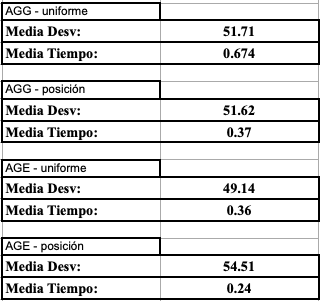
\includegraphics[scale=0.8]{img/gen.png}
\end{figure}

A continuación, desglosamos los resultados para cada caso:
\begin{figure}[H] %con el [H] le obligamos a situar aquí la figura
    \centering
        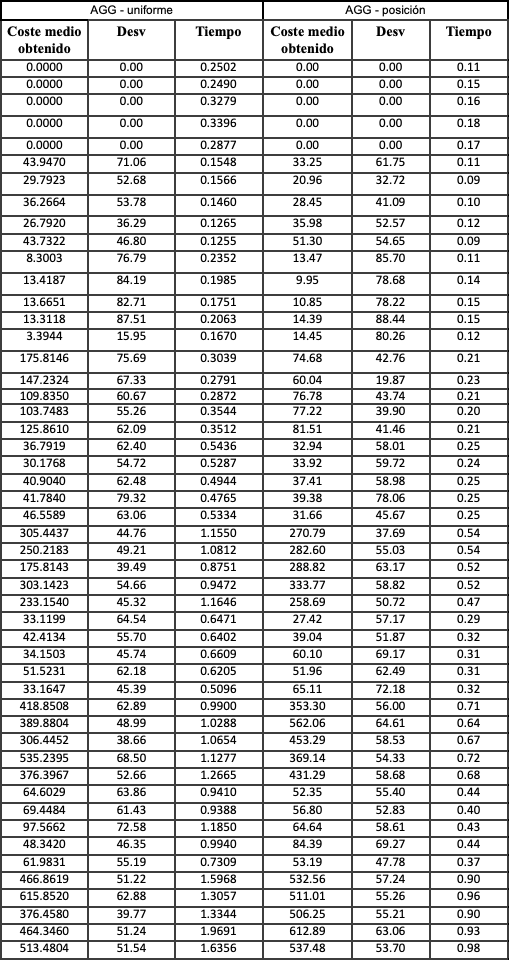
\includegraphics[scale=0.7]{img/agg.png}
\end{figure}
\begin{figure}[H] %con el [H] le obligamos a situar aquí la figura
    \centering
        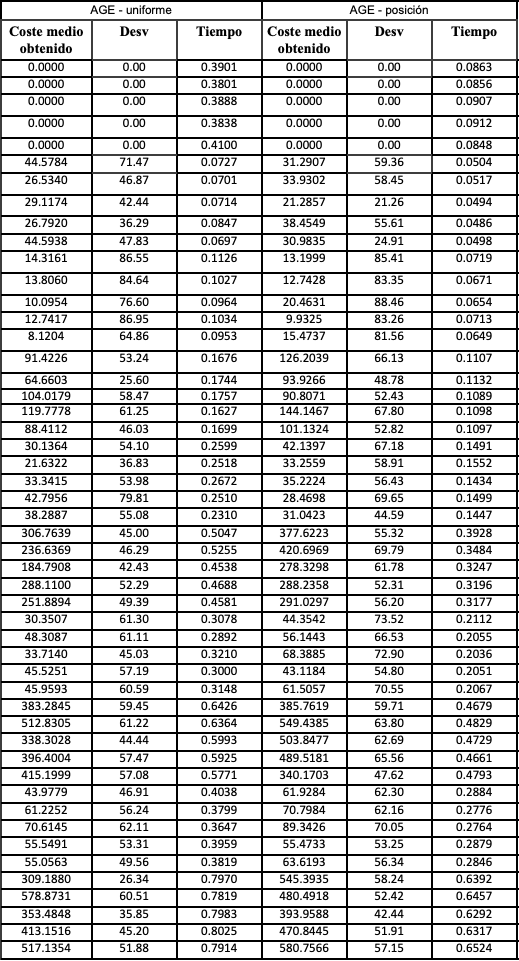
\includegraphics[scale=0.7]{img/age.png}
\end{figure}


\section{Algoritmos Meméticos}
Estos algoritmos surgen de la combinación de los algoritmos genéticos con la búsqueda local. En nuestro caso, utilizamos el algoritmo genético que mejor resultado dio para implementarla (AGE - uniforme). Como se puede observar, en los resultados medios de este problema, los resultados son mejores que con los genéticos en todos los casos.

Especialmente buenos son el algoritmo memético que aplica búsqueda local a toda la población cada 10 iteraciones (AM,1.0) y el que la aplica de forma aleatoria a un 10\% de los individuos que la forman (AM,0.1). Esto puede deberse a que la aleatoriedad y pérdida de buenas soluciones introducida por el algotitmo genético es contrarrestada por la búsqueda local, que analiza el entorno para buscar óptimos locales.

Los tiempos de ejecución también se reducen, ya que la búsqueda local es rápida.

Como desviación y tiempo de ejecución medio entre todos los casos encontramos lo siguiente para cada tipo de algoritmo memético:
\begin{figure}[H] %con el [H] le obligamos a situar aquí la figura
    \centering
        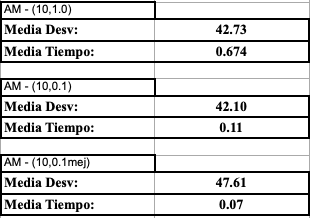
\includegraphics[scale=0.8]{img/mem.png}
\end{figure}

También mostramos los resultados desglosados:
\begin{figure}[H] %con el [H] le obligamos a situar aquí la figura
    \centering
        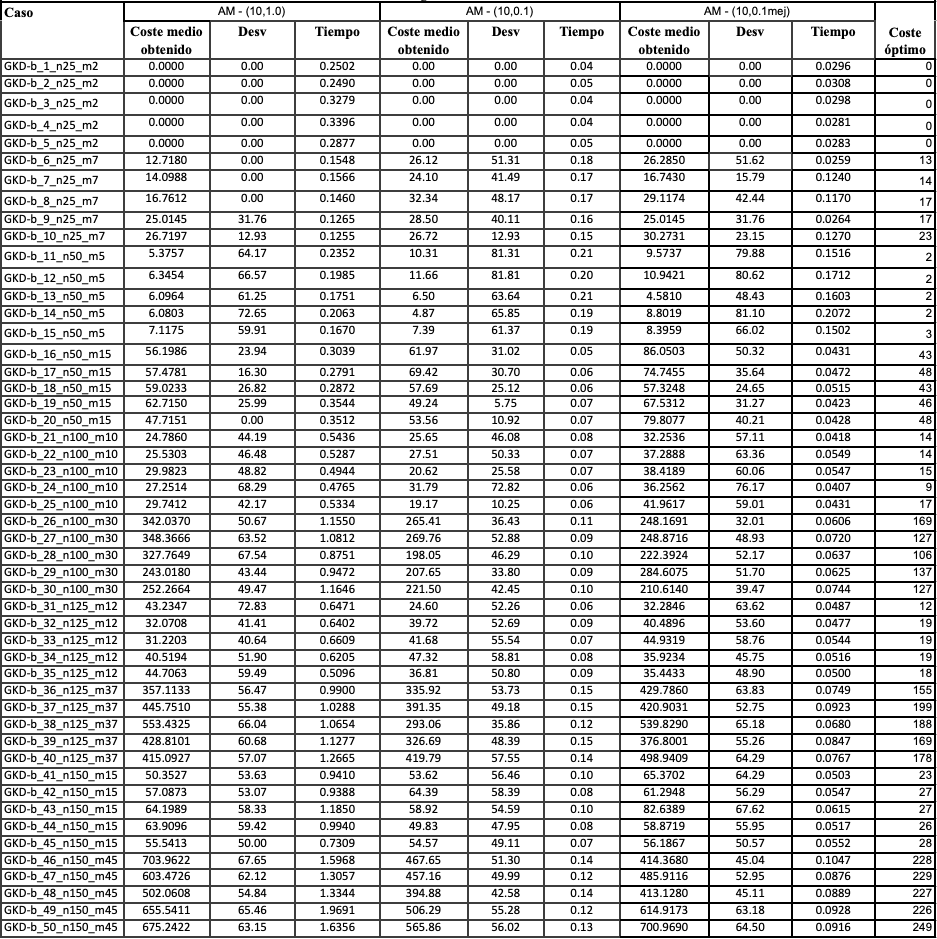
\includegraphics[scale=0.5]{img/am.png}
\end{figure}


%------------------------------------------------
\newpage

\section{Algoritmo Búsqueda Local}
Como referencia, mantenemos los resultados medios de la búsqueda local:
\begin{figure}[H] %con el [H] le obligamos a situar aquí la figura
    \centering
        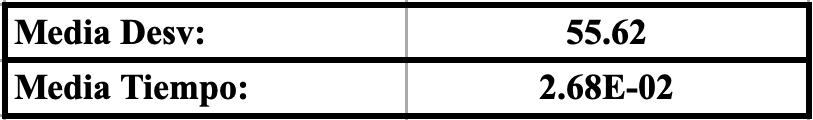
\includegraphics[scale=0.35]{img/bl2.png}
\end{figure}

Los algoritmos genéticos y meméticos mejoran su resultado. Los segundos son especialmente destacables ya que incorporan las ventajas de los genéticos y de la búsqueda local, evitando que quedar atrapados en óptimos locales.

Los algoritmos genéticos tienen una desventaja, y es que según la versión que utilicemos la población puede verse demasiado modificada entre iteración e iteración. Además, la calidad del operador de cruce también afecta seriamente a la de los sucesores.

\begin{figure}[H] %con el [H] le obligamos a situar aquí la figura
    \centering
        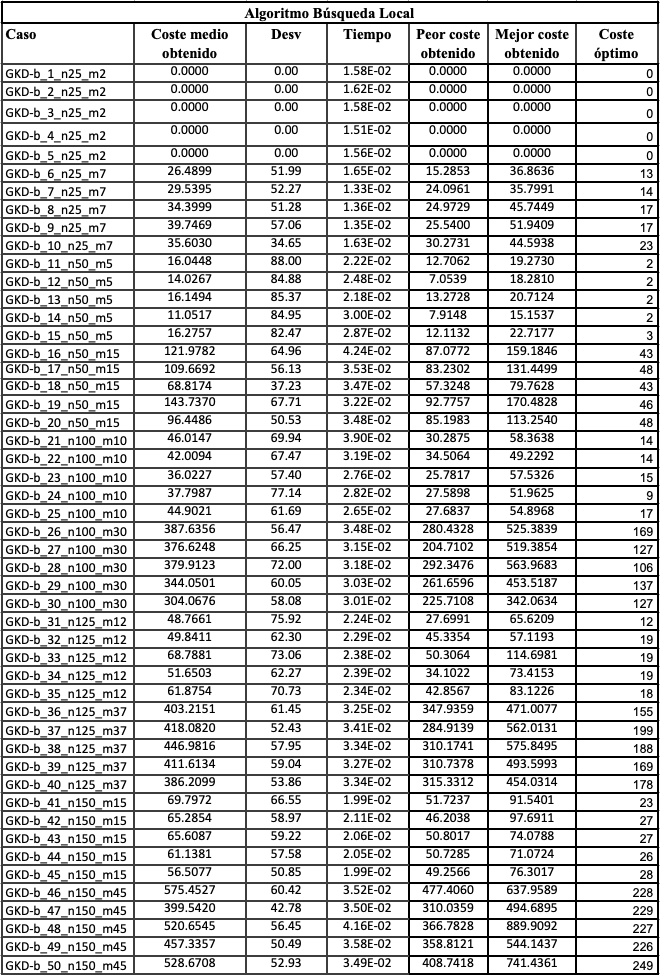
\includegraphics[scale=0.65]{img/bl.png}
\end{figure}

\end{document}


